\documentclass[10pt]{article}
\usepackage[utf8]{inputenc}
\usepackage[activeacute,spanish]{babel}
\usepackage[left=1.5cm,top=1.5cm,right=1.5cm, bottom=1.5cm,letterpaper, includeheadfoot]{geometry}

\usepackage{amssymb, amsmath, amsthm}
\usepackage{graphicx}
\usepackage{hyperref}
\usepackage{lmodern,url}
\usepackage{paralist} %util para listas compactas
\usepackage{xcolor}
\usepackage{bbm}
\usepackage{mathrsfs}
\usepackage{bbm}

%========PAQUETES AGREGADOS===========
%Pseudocodigo
\usepackage{pseudocode}
\usepackage[portuguese, boxruled]{algorithm2e}
\usepackage{wrapfig}
\usepackage{multicol}
\usepackage{graphicx}
\usepackage{caption}
\usepackage{subcaption}
%\captionsetup[table]{labelformat=empty}
\captionsetup[subfigure]{labelformat=empty}
\usepackage{cancel}
\usepackage{tikz}
\def\checkmark{\tikz\fill[scale=0.4](0,.35) -- (.25,0) -- (1,.7) -- (.25,.15) -- cycle;} 
%====================================

\usepackage{fancyhdr}
\pagestyle{fancy}
\fancypagestyle{plain}{%
\fancyhf{}
\lhead{\footnotesize\itshape\bfseries\rightmark}
\rhead{\footnotesize\itshape\bfseries\leftmark}
}


% macros
\newcommand{\Q}{\mathbb Q}
\newcommand{\R}{\mathbb R}
\newcommand{\N}{\mathbb N}
\newcommand{\Z}{\mathbb Z}
\newcommand{\C}{\mathbb C}
\newcommand{\BigO}{\mathcal{O}}
%Teoremas, Lemas, etc.
\theoremstyle{plain}
\newtheorem{teo}{Teorema}
\newtheorem{lem}{Lema}
\newtheorem{prop}{Proposición}
\newtheorem{cor}{Corolario}
\newtheorem{obs}{Observación}
\newtheorem{ej}{Ejemplo}
\renewcommand{\qedsymbol}{\rule{0.7em}{0.7em}}
\renewenvironment{proof}{{\bfseries \noindent Demostración}}{ \qed \\}


\theoremstyle{definition}
\newtheorem{defi}{Definición}
% fin macros


\newcommand{\catnum}{10} %numero de catedra
\newcommand{\fecha}{13 de Septiembre 2016 }

%%%%%%%%%%%%%%%%%%

%Macros para este documento
\newcommand{\cin}{\operatorname{cint}}



\begin{document}
%Encabezado
\fancyhead[L]{Facultad de Ciencias Físicas y Matemáticas}
\fancyhead[R]{Universidad de Chile}
\vspace*{-1.2 cm}
\begin{minipage}{0.6\textwidth}
\begin{flushleft}
\hspace*{-0.5cm}\textbf{MA3402-1 Estadística. Primavera 2016}\\
\hspace*{-0.5cm}\textbf{Profesor:} Raul Gouet\\
\hspace*{-0.5cm}\textbf{Escriba:} Manuel Cáceres\\
\hspace*{-0.5cm}\textbf{Fecha:} \fecha
\end{flushleft}
\end{minipage}
\begin{minipage}{0.36\textwidth}
\begin{flushright}

\includegraphics[scale=0.3]{imagenes/fcfm_dcc}
\end{flushright}
\end{minipage}
\bigskip
%Fin encabezado

\begin{center}
\LARGE\textbf{Clase \catnum}
\end{center}
\section{Test de Neyman-Pearson}
$X_{1}, X_{2}, \ldots, X_{n}$ iid $N(\mu,\sigma)$, $\sigma>0$ conocido.\\
$H_{0}: \mu = \mu_{0}$ versus $H_{1}: \mu = \mu_{1}$ con $\mu_{1}<\mu_{0}$.\\

Encontramos que el TNP de nivel $\alpha$ tiene región crítica dada por :
\begin{align*}
\mathbb{R}^* = \{x\in \mathfrak{X}\colon \underbrace{\bar{X}\ge \mu_{0}+ \frac{\sigma}{\sqrt{n}}\Phi^{-1}(1-\alpha)}_{k_{\alpha}}\}
\end{align*}
La potencia del TNP (en este ejemplo) es $\alpha(\mu_{1}) = \mathbb{P}_{\mu_{1}}(\bar{X}\ge k_{\alpha})$.\\
Bajo $H_{1}$ (cuando calculamos $\mathbb{P}_{\mu_{1}}$) $\bar{X} \sim N(\mu_{1},\frac{\sigma^2}{n})$ y $Z = \frac{\bar{X}-\mu_{1}}{\frac{\sigma}{\sqrt{n}}} \sim N(0,1)$ 
\begin{align*}
\alpha(\mu_{1}) = \mathbb{P}_{\mu_{1}}\left(Z \ge (k_{\alpha}-\mu_{1})\frac{\sqrt{n}}{\sigma}\right) = \underbrace{(1-\Phi)}_{funcion}\left(\frac{\sqrt{n}}{\sigma}\underbrace{(\mu_{0}-\mu_{1})}_{>0}+\Phi^{-1}(1-\alpha)\right)
\end{align*}
\textbf{¿Qué pasa con la potencia cuando... ?}
\begin{itemize}
\item $\alpha \rightarrow 1$, $\alpha(\mu_{1}) \rightarrow 1$
\item $\alpha \rightarrow 0$, $\alpha(\mu_{1}) \rightarrow 0$
\item $\mu_{1} \rightarrow \pm\infty, \alpha(\mu_{1}) \rightarrow 1$
\end{itemize}

\begin{ej} (Bernoulli)\\
$X_{1}, X_{2}, \ldots, X_{n}$ iid, con $\theta \in \{\theta_{0},\theta_{1}\} = \Theta \subseteq [0,1]$.\\
Tenemos $H_{0}: \theta = \theta_{0}$ y $H_{1}: \theta = \theta_{1}$, con $\theta_{1}>\theta_{0}$.
\begin{align*}
\mathbb{R}^* = \{x \in \mathfrak{X} = \{0,1\}^n\colon f_{1}(\lambda) \ge f_{0}(\lambda)k_{\alpha}\}\\
\mathbb{P}_{\theta_{0}}(x \in \mathbb{R}^*) = \alpha, \alpha \in (0,1)\\
f_{0}(x) = \theta^{\sum x_{i}}(1-\theta)^{n-\sum x_{i}} \Rightarrow & \frac{f_{1}(x)}{f_{0}(x)} = \left(\frac{\theta_{1}/(1-\theta_{1})}{\theta_{0}/(1-\theta_{0})}\right)\left(\frac{1-\theta_{0}}{1-\theta_{1}}\right)^n \ge k_{\alpha}\\
\Leftrightarrow & \left(\frac{\theta_{1}/(1-\theta_{1})}{\theta_{0}/(1-\theta_{0})}\right)^{\sum X_{i}} \ge k_{\alpha}'\\
\sum X_{i} \ge k_{\alpha}''
\end{align*}
Sabemos que $\sum X_{i}$ es binomial $\sim B(n,\theta)$, entonces hay que buscar $k_{\alpha}$ tal que 
\begin{align*}
&\mathbb{P}_{\theta_{0}}\left(\sum X_{i} \ge k_{\alpha}''\right) = \alpha\\
\Leftrightarrow &\sum_{k\ge k_{\alpha}''} \binom{n}{k} \theta_{0}^k (1-\theta_{0})^{n-k} = \alpha
\end{align*}
Este $k_{\alpha}''$ puede no existir porque la función no es continua y no existe entonces el TNP de nivel $\alpha$.\\

Dos tipos de soluciones:
\begin{enumerate}
\item \textbf{Práctica}: Cambiar el $\alpha$ por $\tilde{\alpha}<\alpha$, lo más cercano posible y que exista $k_{\alpha}''$
\item \textbf{Matemática}: Usar test ``aleatorizado'' de Neyman-Pearson
\end{enumerate}
Dado un problema $H_{0}: \theta \in \Theta_{0}$ vs $H_{1}: \theta \in \Theta_{1}$, hemos definido como test a cualquier función $\Phi : \mathfrak{X} \mapsto \{0,1\}$.\\

Ahora bien, un test aleatorizado $\Phi_{a}$ es una función $\Phi_{a} : \mathfrak{X} \mapsto [0,1]$. Con esta función se rechaza $H_{0}$ con probabilidad $\Phi_{a}(X)$, habiendo observado $X=x$. Si $Z$ es una variable aleatoria de Bernoulli, tal que $\mathbb{P}_{\theta}(Z=1|X=x)=\Phi_{z}(X)$, rechazamos $H_{0}$ si $Z=1$.
\begin{align*}
\alpha_{\Phi_{a}}(\theta) = \mathbb{P}_{\theta}(Z=1) = \int{\underbrace{\mathbb{P}_{\theta}(Z=1|X=x)}_{\Phi_{a}(X)}f_{\theta}(x) dx} = \mathbb{E}_{\theta}(\Phi_{a}(X))
\end{align*}
Consideremos la clase de los tests aleatoriados de nivel $\alpha$:
\begin{align*}
\tau_{\alpha}^{a} = \{\Phi_{a}: \mathfrak{X}\mapsto [0,1]\colon \alpha_{\Phi_{0}}(\theta)\le \alpha, \forall \theta \in \Theta\} \supseteq \tau_{\alpha}
\end{align*}
El lema de Neyman-Pearson generalizado afirma que siempre existe un test $\tau_{\alpha}^{a}$ de máxima potencia para $H_{0}: \theta = \theta_{0}$ vs $H_{1}: \theta=\theta_{1}$, $\Theta = \{\theta_{0}, \theta_{1}\}$.\\

Este test óptimo tiene el siguiente aspecto:
\begin{align*}
\Phi_{a}^{*}(X) =
\begin{cases} 
      1 & si\ f_{1}(X)>kf_{0}(X) \\
      c \in [0,1]& si\ f_{1}(X)=kf_{0}(X) \\
      0 & si\ f_{1}(X)<kf_{0}(X)
\end{cases}
\end{align*}
, donde $k$ y $c$ se determinan para que $\alpha_{\Phi_{a}^*}(\theta_{0}) = \alpha$\\

La idea para ver $k$ y $c$ es la siguiente.\\
Definimos
\begin{align*}
\beta (k) &= \mathbb{P}_{\theta_{0}}\left(X \in \{X| f_{1}(X) > kf_{0}(X)\}\right)\\
&= \mathbb{P}_{\theta_{0}}\left(\frac{f_{1}(X)}{f_{0}(X)}>k\right) \\
&= 1- \gamma (k)
\end{align*}
, donde $\gamma$ es la función de distribución de la variable aleatoria $\frac{f_{1}(X)}{f_{0}(X)}$.\\
$\Rightarrow \beta (k)$ es continua a la derecha y decreciente a $0$.
\begin{center}
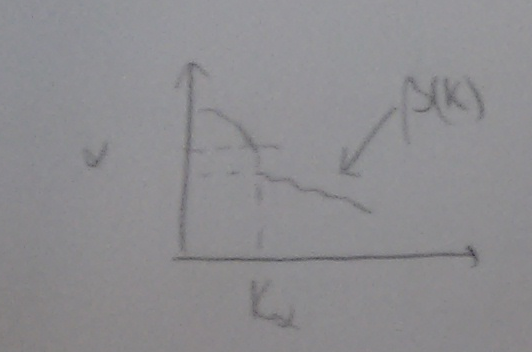
\includegraphics[scale=0.2]{imagenes/aleatorizado.png}
\end{center}
Veamos que $\beta (k_{\alpha}) = \alpha$ no ocurre siempre si $\beta$ es discontinuo.\\

Definamos el valor $\tilde{k_{\alpha}}$ tal que $\beta (\tilde{k_{\alpha}}) \le \alpha \le \beta (\tilde{k_{\alpha}}')$. Y así definimos $c$:
\begin{align*}
c = \frac{\alpha - \beta (\tilde{k_{\alpha}})}{\beta (\tilde{k_{\alpha}}') - \beta (\tilde{k_{\alpha}})}
\end{align*}
Hay que probar que con esta elección de $k$ y $c$ $(\tilde{k_{\alpha}}',c)$ se tiene un test aleatorizado de nivel $\alpha$.
\begin{align*}
\mathbb{E}_{\theta_{0}}(\tilde{\Phi_{a}^*}(X)) &= \underbrace{\mathbb{P}_{\theta_{0}}(f_{1}(X)>\tilde{k_{\alpha}}f_{0}(X))}_{\beta (\tilde{k_{\alpha}})}+ c\cdot\underbrace{\mathbb{P}_{\theta_{0}}(f_{1}(X)=\tilde{k_{\alpha}}f_{0}(X))}_{\beta (\tilde{k_{\alpha}}')-\beta (\tilde{k_{\alpha}})}+ 0\cdot\mathbb{P}_{\theta_{0}}(f_{1}(X)<\tilde{k_{\alpha}}f_{0}(X))\\
&= \alpha
\end{align*}
\end{ej}
Ahora nos enfrentamos a hipótesis compuestas y veremos si el TNP sirve o no sirve.\\
Veamos un caso en que parece que el TNP sea útil:\\
$X_{1},X_{2},\ldots, X_{n}$ iid $\sim N(\mu ,\sigma^2), \sigma>0$ conocido. Sea $\mu_{0} \in \mathbb{R}$.\\

Consideremos $H_{0}: \mu \le \mu_{0}$ vs $H_{1}: \mu > \mu_{0}, \mu \in \mathbb{R}$ o $H_{0}: \mu = \mu_{0}$ vs $H_{1}: \mu > \mu_{0}, \mu \in (\mu_{0}, \infty)$ rechazando cuando $\bar{X}$ es grande.\\

En $H_{0}: \mu \le \mu_{0}$ vs $H_{1}: \mu \not = \mu_{0}, \mu \in \mathbb{R}$ se muere.\\

En $H_{0}: \mu = \mu_{0}$ vs $H_{1}: \mu = \mu_{1}, \mu \in \mathbb{R}$ con $\mu_{1}>\mu_{0}$ rechazamos si $\bar{X}\ge \mu_{0} + \underbrace{\frac{\sigma}{\sqrt{n}}\Phi^{-1}(1-\alpha)}_{\text{no depende de $\mu_{1}$}}$

\end{document}
